\documentclass[10pt,a4paper]{article}

\usepackage[polish]{babel}
\usepackage{polski}
\usepackage[utf8]{inputenc}
\usepackage[T1]{fontenc}
\usepackage[pdftex]{graphicx}
\usepackage{geometry}
\usepackage{chngpage}
\usepackage{indentfirst}
\usepackage{chemstyle}
\usepackage{xymtex}
\usepackage{array, booktabs}
\usepackage{float}
\frenchspacing 
\newcolumntype{x}[1]{>{\centering\arraybackslash}m{#1}} 
\def\lcntNo(#1,#2)#3{\put(#1,#2){\hbox to0pt{\hss\scriptsize #3\hss}}}
\newcolumntype{z}[1]{>{\arraybackslash} p{#1}}
\def\lcntNo(#1,#2)#3{\put(#1,#2){\hbox to0pt{\hss\scriptsize #3\hss}}}
\usepackage{subfig}
\usepackage{amsmath}
\usepackage{setspace}
\frenchspacing 

\title{Zaawansowane technologie w bazach danych\\
Analiza sieci społecznych w portalu last.fm}

\author{  Justyna Plewa \\ Paweł Pierzchała  }

\begin{document}


\maketitle



\newpage

\section {Cel projektu}
Celem projektu jest analiza społeczności tworzących się w portalach internetowych. W analizowanym serwisie wyszukujemy społeczności oraz określamy ich strukturę. 

\section {Portal last.fm}
Last.fm jest internetową radiostacją, system muzycznych rekomendacji oraz portalem społecznościowym. Każdy z użytkowników ma listę odtwarzanych utworów, którą może aktualizować na „żywo” używając plugin-ów do popularnych odtwarzaczy plików mp3. Gromadzone są również dane o koncertach na których bywa użytkownik. Ponad to serwis udostępnia funkcje typowe dla innych portali społecznościowych takie jak znajomi, galerie, komentarze.

Portal udostępnia publiczne dane użytkowników w formacie XML po przez web-service, którego ograniczeniem jest liczba 5 zapytań na sekundę.

W projekcie analizujemy następujące powiązania między użytkownikami:
\begin{itemize}
\item Lista znajomych
\item Ulubione utwory – dwaj użytkownicy są powiązani, jeżeli mają taki sam ulubiony utwór
\item Koncerty – dwaj użytkownicy są powiązani, jeżeli byli na tym samym koncercie
\end{itemize}
Informacje o koncertach udostępniane są wraz z ich terminem, który wykorzystujemy do wyodrębniania głównych członków grup.


\section {Technologie}
Projekt został zaimplementowany w języku Java, z użyciem technologii:

\begin{itemize}
\item Hibernate – do mapowania danych z bazy DB2
\item Jung – wykorzystaliśmy struktury danych, moduł do wizualizacji, alalgorytm klastrujący oraz narzędzia do obliczania miar sieci społecznych
\item Baza danych DB2
\item last.fm API bindings for Java do pobierania danych z portalu Last.fm
\end{itemize}

\subsection {Architektura}
Na załączonej ilustracji widoczne są komponenty projektu oraz komunikacja między nimi.

\begin{figure}[H]
\centering
\caption{Komponenty projektu.}
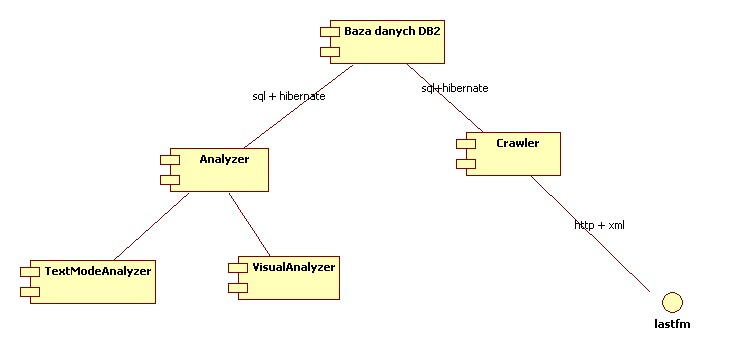
\includegraphics[scale=0.65]{rys1.PNG}
\end{figure}

\subsubsection {Komponent Crawler}
	Komponent Crawler wykorzystuje „last.fm API bindings for Java” do komunikacji z serwisem. Zapewnia on poprawne pobieranie danych po przez protokół HTTP oraz parsowanie plików XML z danymi. Przetworzone dane zapisywane są w bazie danych DB2 znajdującej się na uczelni.
\subsubsection {Komponent Baza Danych DB2}
	Komponent baza danych DB2 umożliwia prosty dostęp danych po przez automatyczne mapowanie klas na rekordy w bazie danych przy pomocy hibernate. Komunikuje się z Crawlerem oraz komponentem Analysis.
\subsubsection {Komponent Analysis}
	Jest to komponent zawierający funkcjonalności niezbędne do przeprowadzenia analiz. Umożliwia generowanie grafów powiązań na podstawie danych z bazy, generowanie raportów oraz analiz.
\subsubsection {Komponent VisualAnlyzer}
	VisualAnalyzer jest graficznym interfejsem do komponentu Analysis. Umożliwia wizualizację sieci oraz sterowanie parametrem klastrowania.
\subsubsection {Komponent TextModeAnalyzer}
	Komponent TextModeAnalyzer jest narzędziem wiersza poleceń które umożliwia generowanie raportów tekstowych z klastrowania.


\subsection {Pobrane dane}
W trakcie semestru pobraliśmy z serwisu last.fm dane o:
\begin{itemize}
\item Użytkownikach – 9826 rekordów
\item Znajomych – 13700 informacji o powiązaniu
\item Utworach – 21 874 rekordów
\item Ulubionych utworach użytkowników – 28 004 rekordów
\item Koncertach – 31 251 rekordów
\item Uczestnikach koncertów – 125 948 powiązań
\end{itemize}
\subsection {Baza danych}
	Struktura bazy danych użyta w projekcie oddaję strukturę powiązań występujących w serwisie last.fm. Poniżej prezentujemy fragment schematu bazy danych który jest używany w projekcie, nie przedstawiamy na nim tabel z których nie korzystaliśmy (np. tabele na tagi lub shouty).

\begin{figure}[H]
\centering
\caption{Struktura bazy danych.}
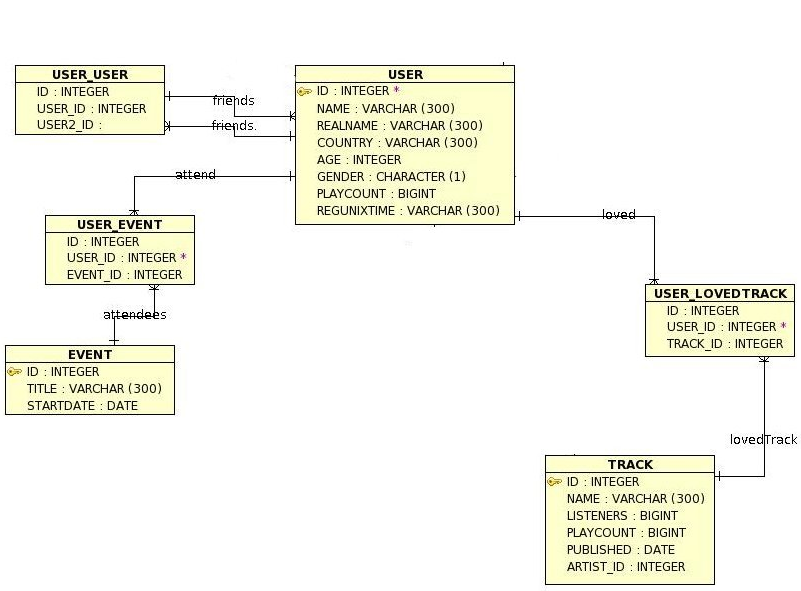
\includegraphics[scale=0.6]{rys2.PNG}
\end{figure}

\subsubsection{Tabela User}
Jeden rekord reprezentuje jedenego użytkownika serwisu Last.fm

% Table generated by Excel2LaTeX from sheet 'Arkusz3'
\begin{table}[H]
  \centering
    \begin{tabular}{cccc}
    \addlinespace
    \toprule
    Nazwa & Typ   & Klucz & Opis \\
    \midrule
    ID    & Integer & Główny & Unikatowy identyfikator użytkownik \\
    NAME  & Varchar(300) &       & Pseudonim użytkownika \\
    REALNAME & Varchar(300) &       & Imię i nazwisko \\
    COUNTRY & Varchar(300) &       & Pochodzenie \\
    AGE   & Integer &       & Wiek użytkownika \\
    GENDER & Character(1) &       & Płeć M/F \\
    REGUNXTIME & Varchar(300) &       & Data rejestracji w formacie unixowym \\
    \bottomrule
    \end{tabular}
  \label{tab:addlabel}
\end{table}

\subsubsection {Tabela User\_User}
Wiąże dwóch użytkowników, reprezentuje powiązanie „Znajomi” z portalu Last.fm.

% Table generated by Excel2LaTeX from sheet 'Arkusz3'
\begin{table}[H]
  \centering
    \begin{tabular}{cccc}
    \addlinespace
    \toprule
    Nazwa & Typ   & Klucz & Opis \\
    \midrule
    ID    & Integer & Główny & Unikatowy identyfikator rekordu \\
    USER\_ID & Integer & Obcy  & Użytkownik pierwszy \\
    USER2\_ID & Integer & Obcy  & Użytkownik drugi \\
    \bottomrule
    \end{tabular}
  \label{tab:addlabel}
\end{table}

\subsubsection {Tabela Event}
Reprezentuje koncert.

% Table generated by Excel2LaTeX from sheet 'Arkusz3'
\begin{table}[H]
  \centering
    \begin{tabular}{cccc}
    \addlinespace
    \toprule
    Nazwa & Typ   & Klucz & Opis \\
    \midrule
    ID    & Integer & Główny & Unikatowy identyfikator koncertu \\
    TITLE & Varchar(300) &       & Nazwa koncertu \\
    STARTDATE & Date  &       & Data rozpoczęcia koncertu \\
    \bottomrule
    \end{tabular}
  \label{tab:addlabel}
\end{table}

\subsubsection {Tabela User\_Event}
Zawiera informację o uczestnikach koncertu.

% Table generated by Excel2LaTeX from sheet 'Arkusz3'
\begin{table}[H]
  \centering
    \begin{tabular}{cccc}
    \addlinespace
    \toprule
    Nazwa & Typ   & Klucz & Opis \\
    \midrule
    ID    & Integer & Główny & Unikatowy identyfikator rekordu \\
    USER\_ID & Integer & Obcy  & Identyfikator użytkownika \\
    EVENT\_ID & Integer & Obcy  & Identyfikator koncertu \\
    \bottomrule
    \end{tabular}
  \label{tab:addlabel}
\end{table}

\subsubsection {Tabela Track}
Tabela Track przechowuje informacje o utworach z serwisu last.fm.

% Table generated by Excel2LaTeX from sheet 'Arkusz3'
\begin{table}[H]
  \centering
    \begin{tabular}{cccc}
    \addlinespace
    \toprule
    Nazwa & Typ   & Klucz & Opis \\
    \midrule
    ID    & Integer & Główny & Unikatowy identyfikator rekordu \\
    NAME  & Integer &       & Nazwa utworu \\
    LISTENERS & BigInt &       & Liczba użytkowników słuchających utworu \\
    PLAYCOUNT & BigInt &       & Liczba odtworzeń utworu \\
    PUBLISHED & Date  &       & Data publikacji \\
    ARTIST\_ID & Integer & Obcy  & Identyfikator autora \\
    \bottomrule
    \end{tabular}
  \label{tab:addlabel}
\end{table}

\subsubsection{Tabela User\_LovedTrack}
W tej tabeli znajdują się powiązania między użytkownikami a ich ulubionymi utworami.

% Table generated by Excel2LaTeX from sheet 'Arkusz3'
\begin{table}[H]
  \centering
    \begin{tabular}{cccc}
    \addlinespace
    \toprule
    Nazwa & Typ   & Klucz & Opis \\
    \midrule
    ID    & Integer & Główny & Unikatowy identyfikator rekordu \\
    USER\_ID & Integer & Obcy  & Identyfikator użytkownika \\
    TRACK\_ID & Integer & Obcy  & Identyfikator utworu \\
    \bottomrule
    \end{tabular}
  \label{tab:addlabel}
\end{table}

\subsection{Problemy}
Początkowo planowaliśmy pobrać dane przy użyciu skryptów napisanych w języku Ruby, okazało się, że plugin którego chcieliśmy użyć nie umożliwiał nam pobrania interesujących nas danych. Zrezygnowaliśmy z Rubego, do pobierania danych wykorzystujemy bibliotekę Javy.

W bibliotece „last.fm API bindings for Java” znajdował się błąd który uniemożliwiał pobieranie koncertów użytkownika z przeszłości. Po pobraniu źródeł biblioteki udało nam się ją naprawić.

\section{Przeprowadzone analizy}
Na podstawie informacji o powiązaniach miedzy użytkownikami tworzony jest nieskierowany graf sieci społecznej. Na tej sieci przeprowadzane jest klastrowanie przy pomocy algorytmu EdgeBetweennessClusterer.

{\itshape EdgeBetweennessClusterer usuwa zadaną liczbę krawędzi o najwyższej wartości Betweenness (po każdorazowym usunięciu miara obliczana jest na nowo). Klastry w tak zredukowanym grafie wyszukiwane są przy użyciu algorytmu WeakComponentClusterer.}

{\itshape WeakComponentClusterer znajduje wszystkie składowe grafy, będące maksymalnym grafami w których między każdą parą wierzchołków istnieje ścieżka wewnątrz.}

Dla każdego wierzchołka grafu obliczane są wartości jego:
\begin{itemize}
\item PageRank – {\itshape określa ważność węzła na podstawie liczności i ważności węzłów doń prowadzących.}
\item Betweenness Centrality – {\itshape istotność węzła jest wyznaczana na podstawie liczby najkrótszych ścieżek przechodzących przez dany węzeł.}
\end{itemize}

Porównujemy wyniki klastrowania różnych sieci powiązań, aby określić ich pokrycie. 
{\itshape Dla dwóch wyników klastrowania A i B, dla każdego klastra z grupy A znajdujemy klaster z grupy B dla którego ich przecięcie jest największe. Określamy stosunek liczebności nowo powstałej grupy i klastra A, który jest pokryciem jednego klastra. Pokrycie jest średnią wszystkich pojedynczych pokryć.}

	Użytkowników do generowania grafów wybierano losowo. Dla tak wybranej próby możemy stworzyć grafy odpowiednich powiązań


\section{Wyniki eksperymentów}

	Poniżej prezentujemy wizualizację oraz analizę różnych grafów dla 200 użytkowników. Każdy z powstałych grafów klastrujemy EdgeBetweennessClustererem usuwając $\frac{1}{5}$, $\frac{2}{5}$, $\frac{3}{5}$ i $\frac{4}{5}$   krawędzi. Dla każdego z tych przypadków prezentujemy wizualizację sieci, tabelę z wartościami miar tej sieci, histogram PageRank oraz BetweennessCentrality. Wynik w którym grupy są widoczne oraz istnieje niewiele grup jedno użytkownikowych jest opisany szczegółowo.


Graf rysowane są w następujący sposób:
\begin{itemize}
	\item Koła oznaczają użytkowników
	\item Ciemne krawędzie oznaczają istniejące połączenia
	\item Jasne krawędzie to krawędzie usunięte w procesie klastrowania
	\item Użytkownicy z tej samej grupy oznaczani są takim samym kolorem
	\item Liczba kolorów jest ograniczona do 10 aby grupy były łatwo rozróżnialne. W sytuacji kiedy jest więcej niż 10 grup ich kolory mogą się powtarzać, natomiast węzły rozmieszcane są tak aby widoczny był brak połączeń ciemnymi krawędziami
\end{itemize} 

\subsection{Klastrowanie Znajomych}

	W tym rozdziale przedstawiamy wyniki klastrowania znajomych, grafu w którym dwaj użytkownicy są połączeni jeżeli są znajomymi w serwisie last.fm. Analizowany graf ma 200 węzłów i 1194 krawędzie.

\subsubsection{Bez usuniętych krawędzi}
	Rysunek poniżej przedstawia sieć znajomych z której nie usunięto jeszcze żadnych krawędzi.

\begin{figure}[H]
\centering
\caption{Graf znajomych bez usuniętych krawędzi.}
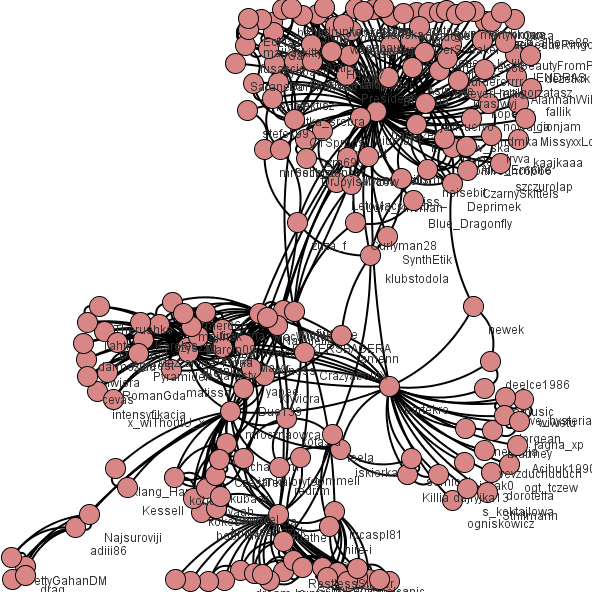
\includegraphics[scale=0.6]{wyniki/final200Friends/0200friends.png}
\label{fig:0200friendsPRHist}
\end{figure}

\begin{figure}[H]
\centering
\caption{Histogram PageRank, 0 usniętych krawędzi}
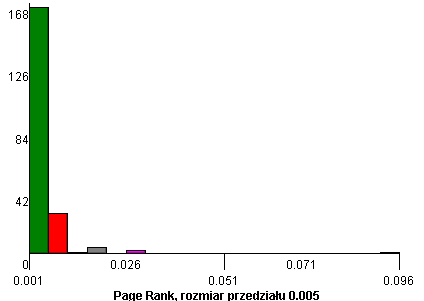
\includegraphics[scale=0.6]{wyniki/final200Friends/0200friendsPRHist.png}
\end{figure}


\begin{figure}[H]
\centering
\caption{Histogram Betweenness Centrality, 0 usniętych krawędzi}
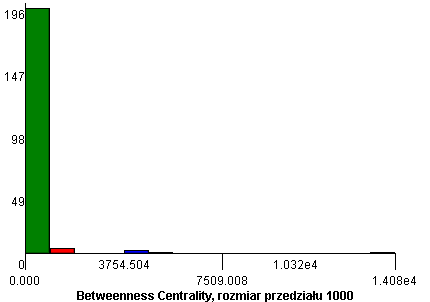
\includegraphics[scale=0.6]{wyniki/final200Friends/0200friendsBCHist.png}
\end{figure}


% Table generated by Excel2LaTeX from sheet 'Arkusz3'
\begin{table}[H]
  \caption{Miary grafu znajomych bez usuniętych krawędzi}
  \centering
    \begin{tabular}{cccc}
    \addlinespace
    \toprule
    Miara & Średnia  & Odchylenie standardowe \\
    \midrule
    Liczba znajomych & 5.97 & 8.76 \\
    PageRank & 0.0050 & 0.0074 \\
    BetweennessCentrality & 185.89 & 1104.93\\ 
    \bottomrule
    \end{tabular}
  \label{tab:addlabel}
\end{table}

Załączone powyżej rysunki przedstawiają normalną strukturę połączeń znajomych występujacych w serwisie last.fm. W tabeli zgromadzone zostały wartości miar sieci społecznych oraz liczbę znajomych, większość użytkowników ma PR oraz BC z najniższego przedziału ponieważ w spójnym grafie będzie kilka głównych wezłów przez które przechodzi większość najkrtótszych ścieżek oraz które mają największy PR.

\subsubsection {Usunięcie $\frac{1}{5}$ krawędzi}
Kolejne ilustracje oraz tabele prezentują wynik klastrowania grafu pozbawionego  $\frac{1}{5}$  krawędzi.
\begin{figure}[H]
\centering
\caption{Graf znajomych po usunięciu $\frac{1}{5}$ krawędzi}
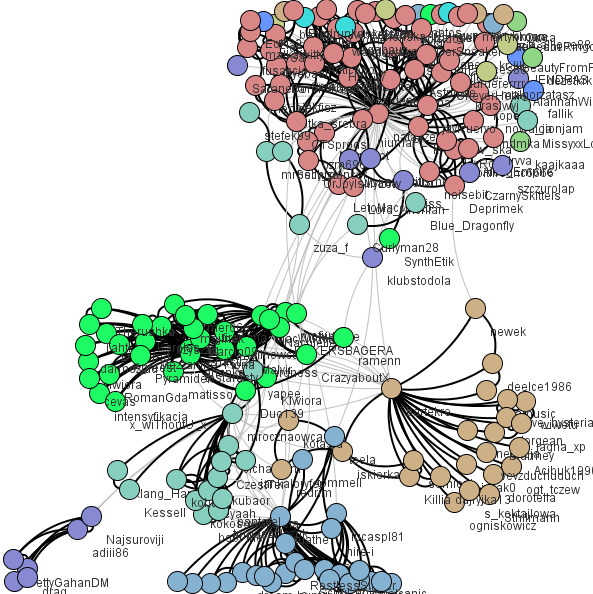
\includegraphics[scale=0.6]{wyniki/final200Friends/1200friends.png}
\end{figure}

\begin{figure}[H]
\centering
\caption{Histogram PageRank, $\frac{1}{5}$ usuniętych krawędzi}
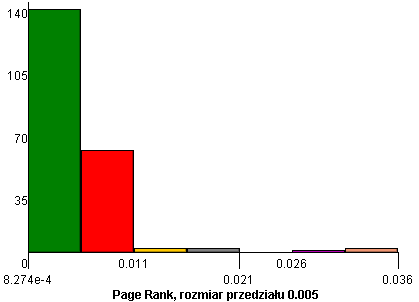
\includegraphics[scale=0.6]{wyniki/final200Friends/1200friendsPRHist.png}
\label{fig:1200friendsPRHist}
\end{figure}


\begin{figure}[H]
\centering
\caption{Histogram Betweenness Centrality $\frac{1}{5}$ usniętych krawędzi}
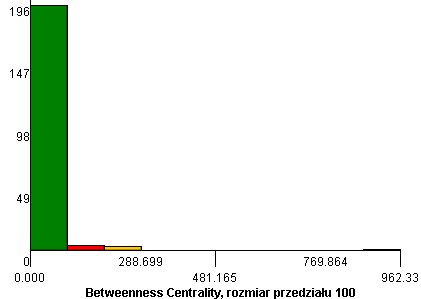
\includegraphics[scale=0.6]{wyniki/final200Friends/1200friendsBCHist.png}
\end{figure}


% Table generated by Excel2LaTeX from sheet 'Arkusz3'
\begin{table}[H]
  \caption{Miary grafu znajomych po usunięciu  $\frac{1}{5}$ usniętych krawędzi}
  \centering
    \begin{tabular}{cccc}
    \addlinespace
    \toprule
    Miara & Średnia  & Odchylenie standardowe \\
    \midrule
    Liczba znajomych & 5.97 & 8.76 \\
    PageRank & 0.0050 & 0.0044 \\
    BetweennessCentrality & 15.04 & 70.73\\ 
    \bottomrule
    \end{tabular}
  \label{tab:frsum15}
\end{table}

\begin{table}[htbp]
\caption{Klastry po usunięci $\frac{1}{5}$ krawędzi }
\begin{center}
\begin{tabular}{x{1.5cm}x{1cm}x{1.7cm}x{2cm}x{1cm}x{2cm}x{1cm}x{2cm}}
    \toprule
Numer klastra & Liczność grupy & Średni stopień węzła & Odchylenie standardowe stopnia węzła & Średnia PR & Odchylenie standardowe PR & Średnia BC & Odchylenie standardowe BC \\ 
\midrule
0 & 54 & 5,8889 & 5,6857 & 0,0055 & 0,0047 & 35,7222 & 122,9039 \\ 
1 & 6 & 2,6667 & 1,5055 & 0,0055 & 0,0028 & 1,1667 & 2,8577 \\ 
2 & 4 & 1,5000 & 0,5774 & 0,0055 & 0,0019 & 1,0000 & 1,1547 \\ 
3 & 1 & 0,0000 & NaN & 0,0008 & NaN & 0,0000 & NaN \\ 
4 & 1 & 0,0000 & NaN & 0,0008 & NaN & 0,0000 & NaN \\ 
5 & 1 & 0,0000 & NaN & 0,0008 & NaN & 0,0000 & NaN \\ 
6 & 27 & 5,2593 & 4,8246 & 0,0055 & 0,0047 & 10,3704 & 47,4897 \\ 
7 & 1 & 0,0000 & NaN & 0,0008 & NaN & 0,0000 & NaN \\ 
8 & 1 & 0,0000 & NaN & 0,0008 & NaN & 0,0000 & NaN \\ 
9 & 34 & 8,3529 & 7,0791 & 0,0055 & 0,0043 & 13,4412 & 38,5630 \\ 
10 & 3 & 1,3333 & 0,5774 & 0,0055 & 0,0022 & 0,3333 & 0,5774 \\ 
11 & 1 & 0,0000 & NaN & 0,0008 & NaN & 0,0000 & NaN \\ 
12 & 2 & 1,0000 & 0,0000 & 0,0055 & 0,0000 & 0,0000 & 0,0000 \\ 
13 & 24 & 3,1667 & 4,0504 & 0,0055 & 0,0066 & 11,4167 & 46,9154 \\ 
14 & 1 & 0,0000 & NaN & 0,0008 & NaN & 0,0000 & NaN \\ 
15 & 1 & 0,0000 & NaN & 0,0008 & NaN & 0,0000 & NaN \\ 
16 & 1 & 0,0000 & NaN & 0,0008 & NaN & 0,0000 & NaN \\ 
17 & 1 & 0,0000 & NaN & 0,0008 & NaN & 0,0000 & NaN \\ 
18 & 1 & 0,0000 & NaN & 0,0008 & NaN & 0,0000 & NaN \\ 
19 & 1 & 0,0000 & NaN & 0,0008 & NaN & 0,0000 & NaN \\ 
20 & 1 & 0,0000 & NaN & 0,0008 & NaN & 0,0000 & NaN \\ 
21 & 1 & 0,0000 & NaN & 0,0008 & NaN & 0,0000 & NaN \\ 
22 & 14 & 6,7143 & 3,0742 & 0,0055 & 0,0022 & 3,1429 & 7,7052 \\ 
23 & 1 & 0,0000 & NaN & 0,0008 & NaN & 0,0000 & NaN \\ 
24 & 2 & 1,0000 & 0,0000 & 0,0055 & 0,0000 & 0,0000 & 0,0000 \\ 
\bottomrule
\end{tabular}
\end{center}
\label{tab:frtab15}
\end{table}

Po usunięciu $\frac{1}{5}$ krawędzi pojawiło się 25 klastrów. Wartości miar dla całego grafu oraz dla poszczególnych klastrów zgromadzone zostały w  \ref{tab:frsum15} oraz \ref{tab:frtab15}. 

W porównaniu z nieklastrowanym grafem można zauwać znaczne zminiejszenie wartości PR i BC, wnika to z rozdzielnie dużego grafu na podgrafy społeczności. Szczególnym przypadkiem, najbardziej zaniżającymi średnie wartości tych miar, są grupy jednoosobowe, BC przyjmuje wartość 0, ponieważ w takim grafie nie ma ścieżek, a PR najniższą możliwą wartość.

Po porównaniu \ref{fig:0200friendsPRHist} oraz \ref{fig:1200friendsPRHist} można zauważyć, zmianę rozkładu PR. W grafie pozbawionym krawędzi, jest znacznie mniej węzłów w najniższym przedziale, dzieje się tak ponieważ, społecznośći w których liczmy te miary są rozłączne, w każdej z nich są węzły z wysokim PR, w grafie niepozbawionym krawędzi jest tylko kilku użytkowników wysokim PR.


\subsubsection {Usunięcie $\frac{2}{5}$ krawędzi}
Kolejne ilustracje oraz tabele prezentują wynik klastrowania grafu pozbawionego  $\frac{2}{5}$  krawędzi.
\begin{figure}[H]
\centering
\caption{Graf znajomych po usunięciu $\frac{2}{5}$ krawędzi}
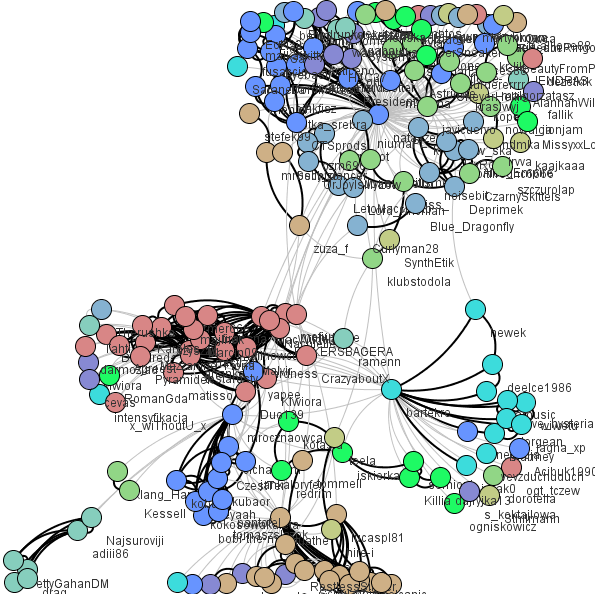
\includegraphics[scale=0.6]{wyniki/final200Friends/2200friends.png}
\end{figure}

\begin{figure}[H]
\centering
\caption{Histogram PageRank, $\frac{2}{5}$ usuniętych krawędzi}
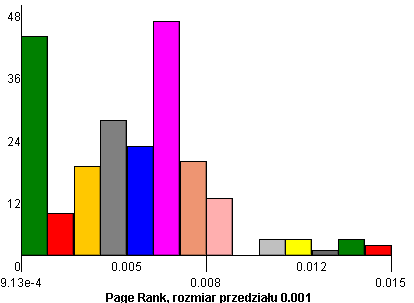
\includegraphics[scale=0.6]{wyniki/final200Friends/2200friendsPRHist.png}
\end{figure}


\begin{figure}[H]
\centering
\caption{Histogram Betweenness Centrality $\frac{3}{5}$ usniętych krawędzi}
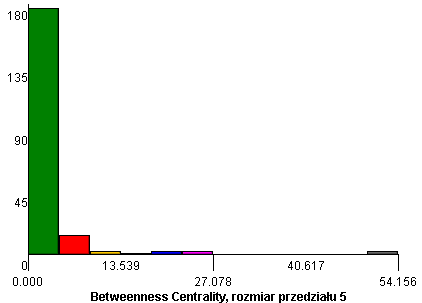
\includegraphics[scale=0.6]{wyniki/final200Friends/2200friendsBCHist.png}
\end{figure}

% Table generated by Excel2LaTeX from sheet 'Arkusz3'
\begin{table}[H]
  \caption{Miary grafu znajomych po usunięciu  $\frac{2}{5}$ usniętych krawędzi}
  \centering
    \begin{tabular}{cccc}
    \addlinespace
    \toprule
    Miara & Średnia  & Odchylenie standardowe \\
    \midrule
    Liczba znajomych & 5.97 & 8.76 \\
    PageRank & 0.0050 & 0.0030 \\
    BetweennessCentrality & 2.03 & 6.18\\ 
    \bottomrule
    \end{tabular}
  \label{tab:addlabel}
\end{table}

Po usunięciu $\frac{2}{5}$ krawędzi powstało 68 klastrów. Społeczności wydzielone w ten sposób nie tworzą już tak zwartych struktur jak w przypadku usuwania $\frac{1}{5}$ krawędzi. Jest coraz mniej użytkowników o dominującej wartości Page Rank, jest to spowodowanem rozbiciem struktur społecznych, istnieją teraz tylko jednostki wpływowe w ramach jednej społeczności a nie całej populacji. Zmniejszyła się również liczba użytkowników z dominującym Betweenes Centrality, wynika to również z podziału grup społecznych, nie ma użytkowników przez których przechodziło by wiele najkrótszych ścieżek.

\subsubsection {Usunięcie $\frac{3}{5}$ krawędzi}
Kolejne ilustracje oraz tabele prezentują wynik klastrowania grafu pozbawionego  $\frac{3}{5}$  krawędzi.
\begin{figure}[H]
\centering
\caption{Graf znajomych po usunięciu $\frac{3}{5}$ krawędzi}
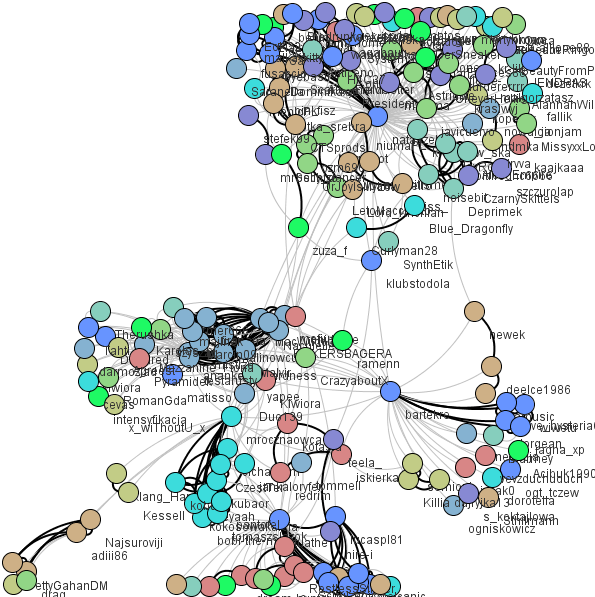
\includegraphics[scale=0.6]{wyniki/final200Friends/3200friends.png}
\end{figure}

\begin{figure}[H]
\centering
\caption{Histogram PageRank, $\frac{3}{5}$ usuniętych krawędzi}
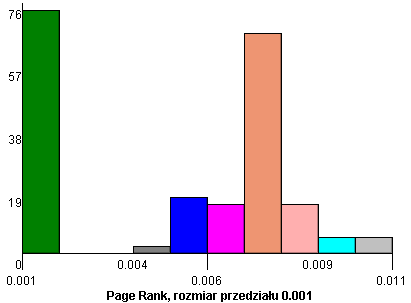
\includegraphics[scale=0.6]{wyniki/final200Friends/3200friendsPRHist.png}
\end{figure}


\begin{figure}[H]
\centering
\caption{Histogram Betweenness Centrality $\frac{3}{5}$ usuniętych krawędzi}
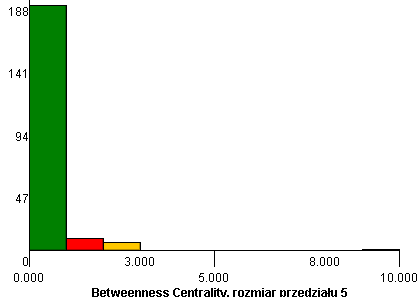
\includegraphics[scale=0.6]{wyniki/final200Friends/3200friendsBCHist.png}
\end{figure}

% Table generated by Excel2LaTeX from sheet 'Arkusz3'
\begin{table}[H]
  \caption{Miary grafu znajomych po usunięciu  $\frac{3}{5}$ krawędzi}
  \centering
    \begin{tabular}{cccc}
    \addlinespace
    \toprule
    Miara & Średnia  & Odchylenie standardowe \\
    \midrule
    Liczba znajomych & 5.97 & 8.76 \\
    PageRank & 0.0050 & 0.0031 \\
    BetweennessCentrality & 0.28 & 0.85\\ 
    \bottomrule
    \end{tabular}
  \label{tab:addlabel}
\end{table}

Pozbawienie grafu $\frac{3}{5}$ krawędzie spowodowało powstanie 106 grup. Można zauważyć bardzo małe zakres wartości miary Page Rank i Betweenes Centrality, tak jak w przypadku $\frac{2}{5}$ jest to spowodowane zmieniejszeniem liczności wydzielonych społeczności.

\subsubsection {Usunięcie $\frac{4}{5}$ krawędzi}
Kolejne ilustracje oraz tabele prezentują wynik klastrowania grafu pozbawionego  $\frac{4}{5}$  krawędzi.
\begin{figure}[H]
\centering
\caption{Graf znajomych po usunięciu $\frac{4}{5}$ krawędzi}
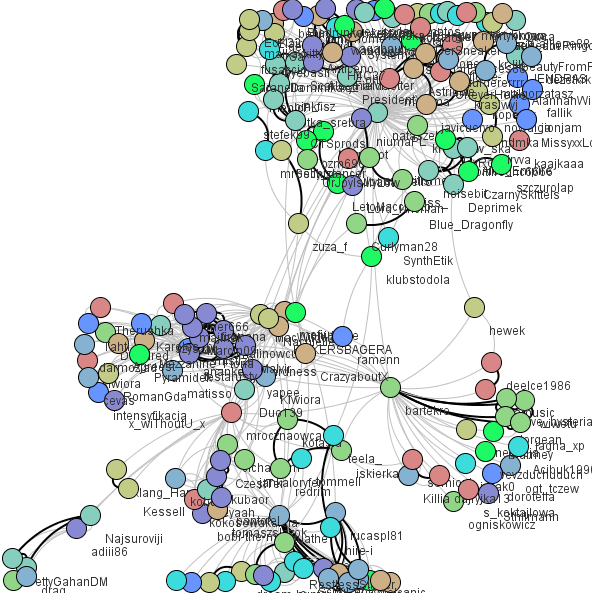
\includegraphics[scale=0.6]{wyniki/final200Friends/4200friends.png}
\end{figure}

\begin{figure}[H]
\centering
\caption{Histogram PageRank, $\frac{4}{5}$ usuniętych krawędzi}
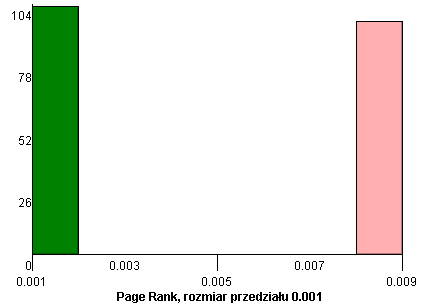
\includegraphics[scale=0.6]{wyniki/final200Friends/4200friendsPRHist.png}
\end{figure}


\begin{figure}[H]
\centering
\caption{Histogram Betweenness Centrality $\frac{4}{5}$ usuniętych krawędzi}
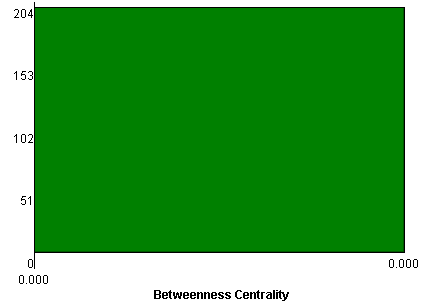
\includegraphics[scale=0.6]{wyniki/final200Friends/4200friendsBCHist.png}
\end{figure}


% Table generated by Excel2LaTeX from sheet 'Arkusz3'
\begin{table}[H]
  \caption{Miary grafu znajomych po usunięciu  $\frac{4}{5}$ krawędzi}
  \centering
    \begin{tabular}{cccc}
    \addlinespace
    \toprule
    Miara & Średnia  & Odchylenie standardowe \\
    \midrule
    Liczba znajomych & 5.97 & 8.76 \\
    PageRank & 0.0050 & 0.0038
 \\
    BetweennessCentrality & 0.0 & 0.0\\ 
    \bottomrule
    \end{tabular}
  \label{tab:addlabel}
\end{table}

Usunięcie $\frac{4}{5}$ połączeń między użytkownikami doprowadziło do powstania 136 klastrów. 
\subsubsection {Wnioski}


\subsection {Klastrowanie Ulubionych}
  W tym rozdziale przedstawiamy wyniki klastrowania znajomych, grafu w którym dwaj użytkownicy są połączeni jeżeli oboje lubią ten sam utwór w serwisie last.fm. Analizowany graf ma 200 węzłów i 1076 krawędzi.
\subsubsection {Bez usuniętych krawędzi}
  Kolejne ilustracje oraz tabele prezentują wynik klastrowania grafu bez usuniętych krawędzi.
\begin{figure}[H]
\centering
\caption{Graf ulubionych, bez usuniętych krawędzi}
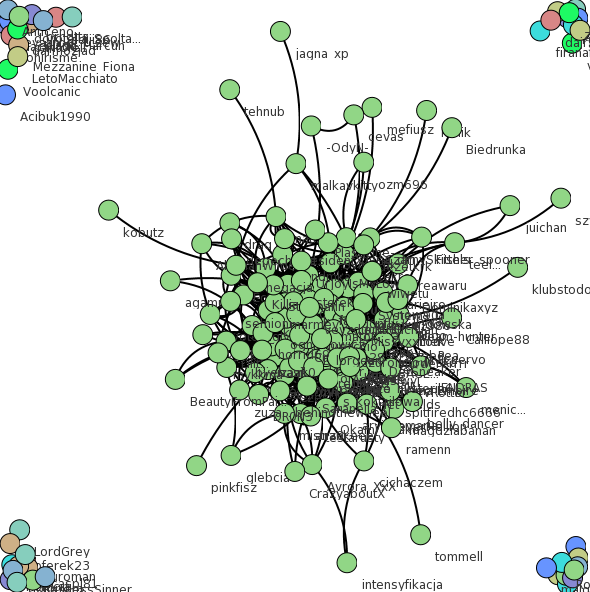
\includegraphics[scale=0.5]{wyniki/final200Loved/0200loved.png}
\end{figure}

\begin{figure}[H]
\centering
\caption{Histogram PageRank, bez usuniętych krawędzi}
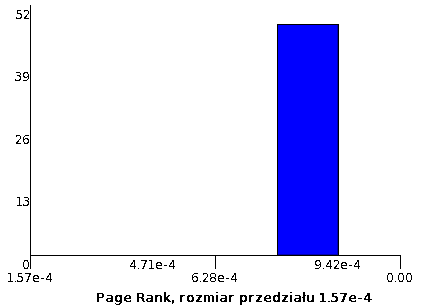
\includegraphics[scale=0.6]{wyniki/final200Loved/0200lovedPRHist.png}
\label{fig:1200lovedPRHist}
\end{figure}


\begin{figure}[H]
\centering
\caption{Histogram Betweenness Centrality, bez usuniętych krawędzi}
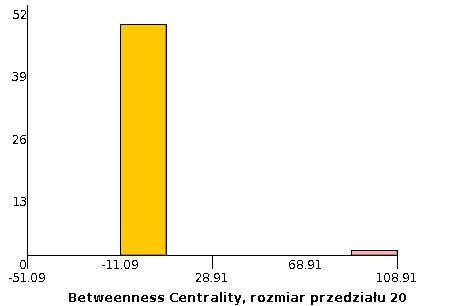
\includegraphics[scale=0.6]{wyniki/final200Loved/0200lovedBCHist.png}
\end{figure}


\begin{table}[H]
  \caption{Miary grafu ulubionych  bez usuniętych krawędzi}
  \centering
    \begin{tabular}{cccc}
    \addlinespace
    \toprule
    Miara & Średnia  & Odchylenie standardowe \\
    \midrule
    Liczba znajomych & 10.76 & 10.53 \\
    PageRank & 0.0050 & 0.0039 \\
    BetweennessCentrality & 77.65 & 109.65\\ 
    \bottomrule
    \end{tabular}
  \label{tab:addlabel}
\end{table}
\begin{verse}
 \centering
    Uwaga: Średni stopień wierzchołka w grafie wynosi 0,2889.
\end{verse}

  



\subsubsection {$\frac{1}{5}$ krawędzi}
  Kolejne ilustracje oraz tabele prezentują wynik klastrowania grafu pozbawionego  $\frac{1}{5}$  krawędzi.
\begin{figure}[H]
\centering
\caption{Graf ulubionych po usunięciu $\frac{1}{5}$ krawędzi}
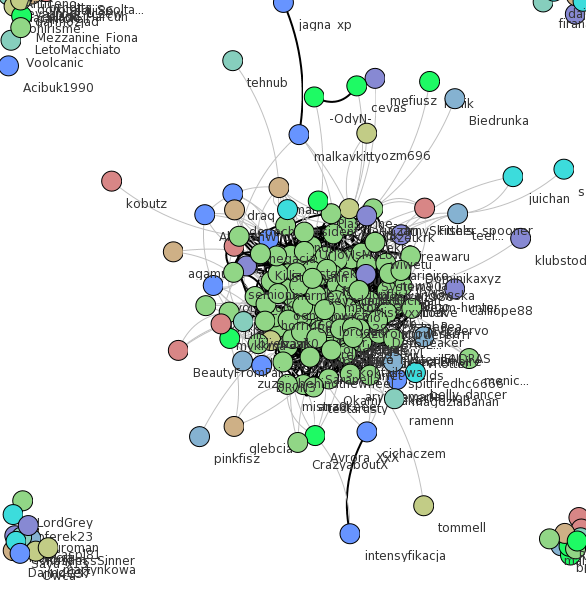
\includegraphics[scale=0.5]{wyniki/final200Loved/1200loved.png}
\end{figure}

\begin{figure}[H]
\centering
\caption{Histogram PageRank, $\frac{1}{5}$ usuniętych krawędzi}
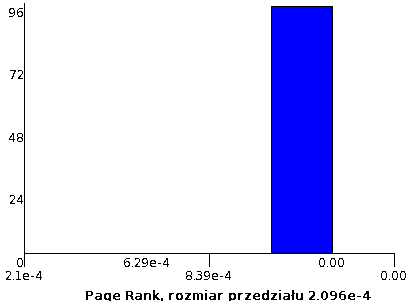
\includegraphics[scale=0.6]{wyniki/final200Loved/1200lovedPRHist.png}
\label{fig:1200lovedPRHist}
\end{figure}


\begin{figure}[H]
\centering
\caption{Histogram Betweenness Centrality $\frac{1}{5}$ usuniętych krawędzi}
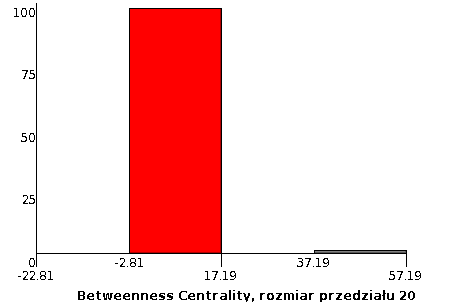
\includegraphics[scale=0.6]{wyniki/final200Loved/1200lovedBCHist.png}
\end{figure}


\begin{table}[H]
  \caption{Miary grafu ulubionych po usunięciu $\frac{1}{5}$ krawędzi}
  \centering
    \begin{tabular}{cccc}
    \addlinespace
    \toprule
    Miara & Średnia  & Odchylenie standardowe \\
    \midrule
    Liczba znajomych & 35.58 & 22.58 \\
    PageRank & 0.0050 & 0.0042 \\
    BetweennessCentrality & 22.58 & 35.58\\ 
    \bottomrule
    \end{tabular}
  \label{tab:frsum22}
\end{table}


Po usunięciu $\frac{1}{5}$ krawędzi powstało 99 klastrów. Wartości miar dla całego grafu zostały przedstawione w  \ref{tab:frsum22}.
\subsubsection {$\frac{2}{5}$ krawędzi}
  Kolejne ilustracje oraz tabele prezentują wynik klastrowania grafu pozbawionego  $\frac{2}{5}$  krawędzi.
\begin{figure}[H]
\centering
\caption{Graf ulubionych po usunięciu $\frac{2}{5}$ krawędzi}
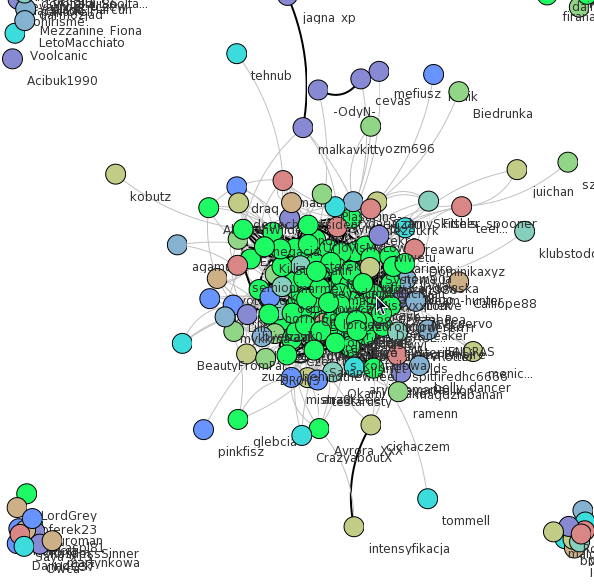
\includegraphics[scale=0.5]{wyniki/final200Loved/2200loved.png}
\end{figure}

\begin{figure}[H]
\centering
\caption{Histogram PageRank, $\frac{2}{5}$ usuniętych krawędzi}
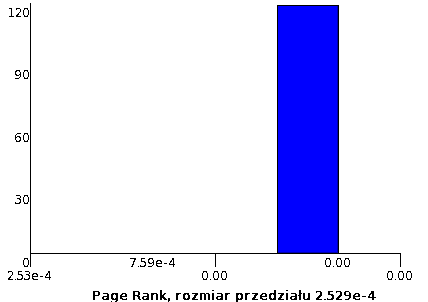
\includegraphics[scale=0.6]{wyniki/final200Loved/2200lovedPRHist.png}
\label{fig:1200lovedPRHist}
\end{figure}


\begin{figure}[H]
\centering
\caption{Histogram Betweenness Centrality $\frac{2}{5}$ usuniętych krawędzi}
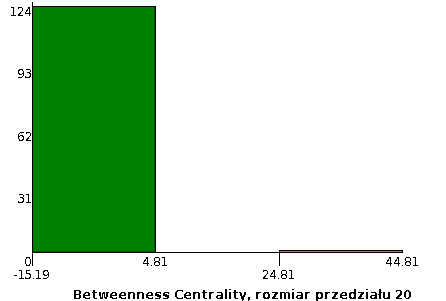
\includegraphics[scale=0.6]{wyniki/final200Loved/2200lovedBCHist.png}
\end{figure}


\begin{table}[H]
  \caption{Miary grafu ulubionych po usunięciu $\frac{2}{5}$ krawędzi}
  \centering
    \begin{tabular}{cccc}
    \addlinespace
    \toprule
    Miara & Średnia  & Odchylenie standardowe \\
    \midrule
    Liczba znajomych & 20.83 & 11.40 \\
    PageRank & 0.0050 & 0.0047 \\
    BetweennessCentrality & 11.40 & 20.83 \\ 
    \bottomrule
    \end{tabular}
  \label{tab:addlabel}
\end{table}

Po usunięciu $\frac{2}{5}$ krawędzi powstały 123 klastry.

\subsubsection {$\frac{3}{5}$ krawędzi}

  Kolejne ilustracje oraz tabele prezentują wynik klastrowania grafu pozbawionego  $\frac{3}{5}$  krawędzi.
\begin{figure}[H]
\centering
\caption{Graf ulubionych po usunięciu $\frac{3}{5}$ krawędzi}
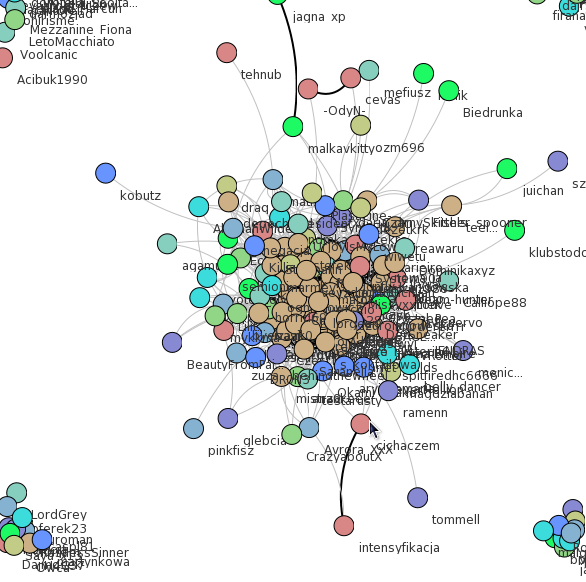
\includegraphics[scale=0.5]{wyniki/final200Loved/3200loved.png}
\end{figure}

\begin{figure}[H]
\centering
\caption{Histogram PageRank, $\frac{3}{5}$ usuniętych krawędzi}
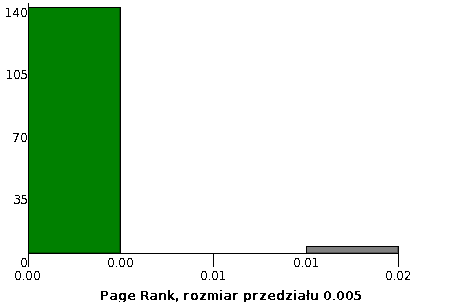
\includegraphics[scale=0.6]{wyniki/final200Loved/3200lovedPRHist.png}
\label{fig:1200lovedPRHist}
\end{figure}


\begin{figure}[H]
\centering
\caption{Histogram Betweenness Centrality $\frac{3}{5}$ usuniętych krawędzi}
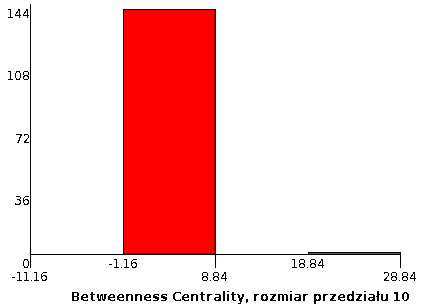
\includegraphics[scale=0.6]{wyniki/final200Loved/3200lovedBCHist.png}
\end{figure}


\begin{table}[H]
  \caption{Miary grafu ulubionych po usunięciu $\frac{3}{5}$ krawędzi}
  \centering
    \begin{tabular}{cccc}
    \addlinespace
    \toprule
    Miara & Średnia  & Odchylenie standardowe \\
    \midrule
    Liczba znajomych & 10.76 & 10.53 \\
    PageRank & 0.0050 & 0.0052 \\
    BetweennessCentrality & 6.25 & 14.10\\ 
    \bottomrule
    \end{tabular}
  \label{tab:addlabel}
\end{table}

Po usunięciu $\frac{3}{5}$ krawędzi powstało 142 klastry. 

\subsubsection {$\frac{4}{5}$ krawędzi}

  Kolejne ilustracje oraz tabele prezentują wynik klastrowania grafu pozbawionego  $\frac{4}{5}$  krawędzi.
\begin{figure}[H]
\centering
\caption{Graf ulubionych po usunięciu $\frac{4}{5}$ krawędzi}
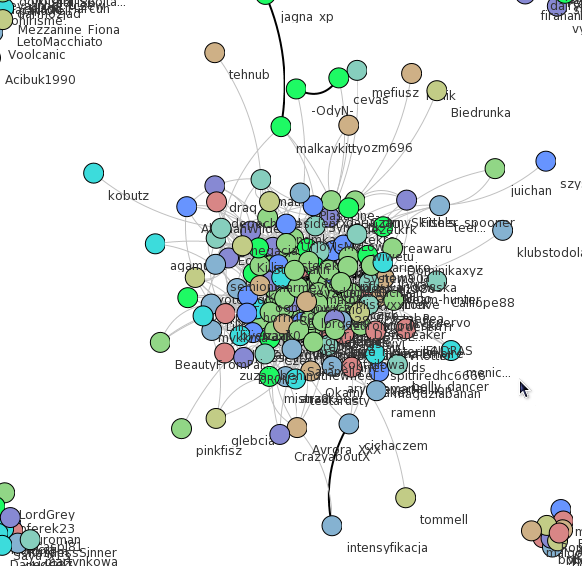
\includegraphics[scale=0.5]{wyniki/final200Loved/4200loved.png}
\end{figure}

\begin{figure}[H]
\centering
\caption{Histogram PageRank, $\frac{4}{5}$ usuniętych krawędzi}
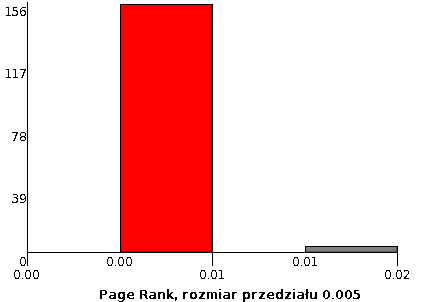
\includegraphics[scale=0.6]{wyniki/final200Loved/4200lovedPRHist.png}
\label{fig:1200lovedPRHist}
\end{figure}


\begin{figure}[H]
\centering
\caption{Histogram Betweenness Centrality $\frac{4}{5}$ usuniętych krawędzi}
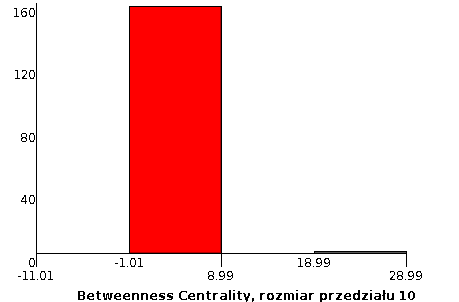
\includegraphics[scale=0.6]{wyniki/final200Loved/4200lovedBCHist.png}
\end{figure}


\begin{table}[H]
  \caption{Miary grafu ulubionych po usunięciu $\frac{4}{5}$ krawędzi}
  \centering
    \begin{tabular}{cccc}
    \addlinespace
    \toprule
    Miara & Średnia  & Odchylenie standardowe \\
    \midrule
    Liczba znajomych & 10.76 & 10.53 \\
    PageRank & 0.0050 & 0.0055 \\
    BetweennessCentrality & 4.30 & 13.50\\ 
    \bottomrule
    \end{tabular}
  \label{tab:addlabel}
\end{table}

Po usunięciu $\frac{1}{5}$ krawędzi powstało 159 klastrów. 

\subsubsection {Wnioski}
Zmniejszanie liczby krawędzi w grafie nie powoduje widocznego tworzenia się klastrów, a jedynie zwiększanie się liczby niepołączonych wierzchołków. 
Spowodowane jest to ogromną ilością utworów, które mogą łączyć użytkowników, w związku z czym zazwyczaj wierzchołek jest połączony tylko z jednym innym wierzchołkiem.
Świadczy o tym niski średni stopień wierzchołka podany w części 5.2.1. Warto zaznaczyć, że ilość wspólnie lubianych utworów nie zmienia, ani ilości połączeń między danymi użytkownikami, ani ich siły.
 


\subsection{Klastrowanie Koncertów}
 W tym rozdziale przedstawiamy wyniki klastrowania koncertów, grafu w którym dwaj użytkownicy są połączeni jeżeli chcą uczestniczyć w tym samym wydarzeniu(np. koncercie), o którym informacja znajduje się w serwisie last.fm. Analizowany graf ma 200 węzłów i 1047 krawędzi.

\subsubsection {Bez usuniętych krawędzi}
  Kolejne ilustracje oraz tabele prezentują wynik klastrowania grafu bez usuniętych krawędzi.
\begin{figure}[H]
\centering
\caption{Graf ulubionych, bez usuniętych krawędzi}
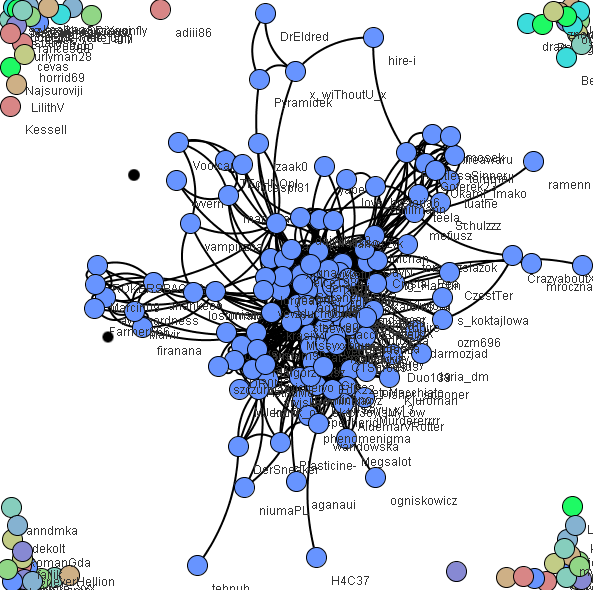
\includegraphics[scale=0.5]{wyniki/final200Events/0200events.png}
\end{figure}

\begin{figure}[H]
\centering
\caption{Histogram PageRank, bez usuniętych krawędzi}
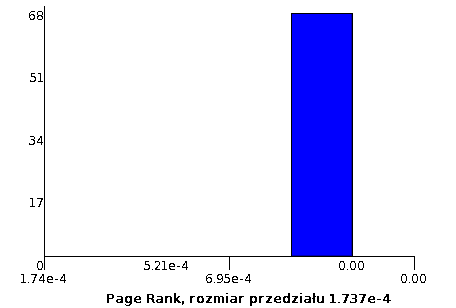
\includegraphics[scale=0.6]{wyniki/final200Events/0200eventsPRHist.png}
\label{fig:1200lovedPRHist}
\end{figure}


\begin{figure}[H]
\centering
\caption{Histogram Betweenness Centrality, bez usuniętych krawędzi}
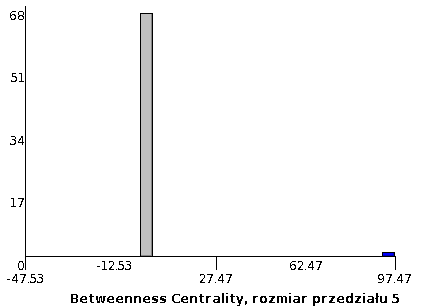
\includegraphics[scale=0.6]{wyniki/final200Events/0200eventsBCHist.png}
\end{figure}


\begin{table}[H]
  \caption{Miary grafu koncertów  bez usuniętych krawędzi}
  \centering
    \begin{tabular}{cccc}
    \addlinespace
    \toprule
    Miara & Średnia  & Odchylenie standardowe \\
    \midrule
    Liczba znajomych & 10.47 & 13.32 \\
    PageRank & 0.0050 & 0.0047 \\
    BetweennessCentrality & 63.69 & 149.30\\ 
    \bottomrule
    \end{tabular}
  \label{tab:addlabel}
\end{table}

\subsubsection {$\frac{1}{5}$ krawędzi}
  Kolejne ilustracje oraz tabele prezentują wynik klastrowania grafu pozbawionego  $\frac{1}{5}$  krawędzi.
\begin{figure}[H]
\centering
\caption{Graf koncertów po usunięciu $\frac{1}{5}$ krawędzi}
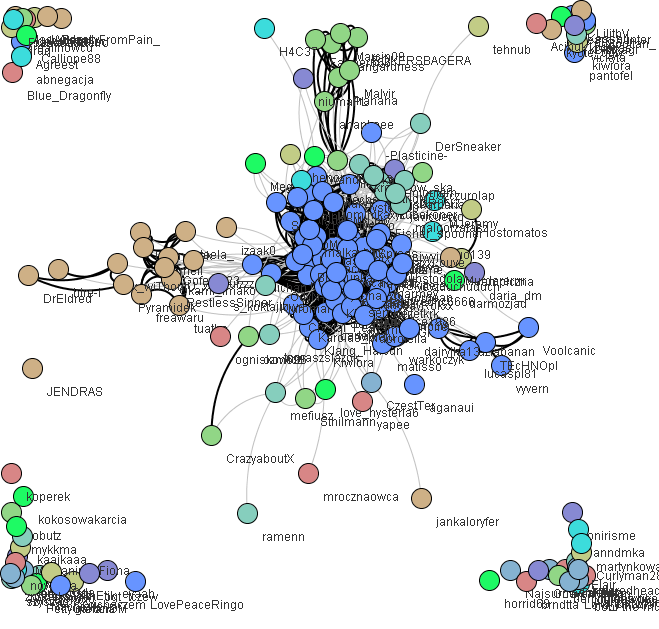
\includegraphics[scale=0.5]{wyniki/final200Events/1200events.png}
\end{figure}

\begin{figure}[H]
\centering
\caption{Histogram PageRank, $\frac{1}{5}$ usuniętych krawędzi}
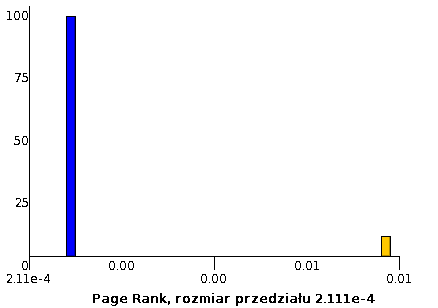
\includegraphics[scale=0.6]{wyniki/final200Events/1200eventsPRHist.png}
\label{fig:1200lovedPRHist}
\end{figure}


\begin{figure}[H]
\centering
\caption{Histogram Betweenness Centrality $\frac{1}{5}$ usuniętych krawędzi}
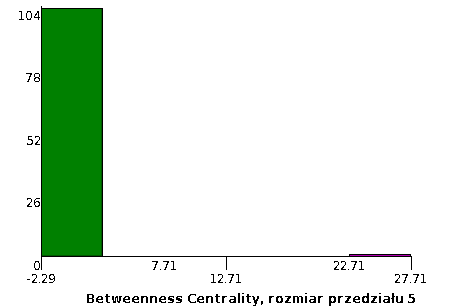
\includegraphics[scale=0.6]{wyniki/final200Events/1200eventsBCHist.png}
\end{figure}


\begin{table}[H]
  \caption{Miary grafu koncertów po usunięciu $\frac{1}{5}$ krawędzi}
  \centering
    \begin{tabular}{cccc}
    \addlinespace
    \toprule
    Miara & Średnia  & Odchylenie standardowe \\
    \midrule
    Liczba znajomych & 10.47 & 13.32 \\
    PageRank & 0.0050 & 0.0042 \\
    BetweennessCentrality & 7.77 & 20.55\\ 
    \bottomrule
    \end{tabular}
  \label{tab:frsum31}
\end{table}

\begin{table}[htbp]
\caption{Wybrane klastry po usunięci $\frac{1}{5}$ krawędzi }
\begin{center}
\begin{tabular}{x{1.5cm}x{1cm}x{1.7cm}x{2cm}x{1cm}x{2cm}x{1cm}x{2cm}}
    \toprule
Numer klastra & Liczność grupy & Średni stopień węzła & Odchylenie standardowe stopnia węzła & Średnia PR & Odchylenie standardowe PR & Średnia BC & Odchylenie standardowe BC \\ 
\midrule
27 & 67 & 22,5672 & 11,2388 & 0,0084 & 0,0036 & 22,8806 & 30,3968 \\ 
33 & 9 & 5,5556 & 1,8105 & 0,0084 & 0,0024 & 1,2223 & 1,7159 \\ 
75 & 8 & 5,7500 & 1,2817 & 0,0084 & 0,0017 & 0,625 & 0,6220 \\ 
102 & 7 & 6,0000 & 0,0000 & 0,0084 & 1,87E-18 & 0,0000 & 0,0000 \\ 
97 & 5 & 2,8000 & 1,0954 & 0,0084 & 0,0029 & 0,6000 & 1,3416 \\ 
103 & 4 & 2,0000 & 0,8165 & 0,0084 & 0,0031 & 0,5000 & 1,0000 \\ 
5 & 2 & 1,0000 & 0,0000 & 0,0084 & 0,0000 & 0,0000 & 0,0000 \\ 
94 & 2 & 1,0000 & 0,0000 & 0,0008 & NaN & 0,0000 & NaN \\ 
8 & 1 & 0,0000 & 0,0000 & 0,0084 & 0,0000 & 0,0000 & 0,0000 \\ 
95 & 1 & 0,0000 & NaN & 0,0013 & NaN & 0,0000 & NaN \\ 
10 & 1 & 0,0000 & NaN & 0,0013 & NaN & 0,0000 & NaN \\ 
11 & 1 & 0,0000 & NaN & 0,0013 & NaN & 0,0000 & NaN \\ 
\bottomrule
\end{tabular}
\end{center}
\label{tab:frtab32}
\end{table}

  Po usunięci $\frac{1}{5}$ krawędzi utworzone zostały 104 klastry. Większość z nich zawiera jedynie po jednym obiekcie, jednakże można zauważyć ok. 10 większych. 
Dane dotyczące całego grafu zawiera  \ref{tab:frsum31}, natomiast te dotyczące największych klastrów  \ref{tab:frtab32}. 
Zauważalne jest zmniejszenie parametru BC spowodowane podziałem dużego grafu na podgrafy społeczności.

\subsubsection {$\frac{2}{5}$ krawędzi}
  Kolejne ilustracje oraz tabele prezentują wynik klastrowania grafu pozbawionego  $\frac{2}{5}$  krawędzi.
\begin{figure}[H]
\centering
\caption{Graf koncertów po usunięciu $\frac{2}{5}$ krawędzi}
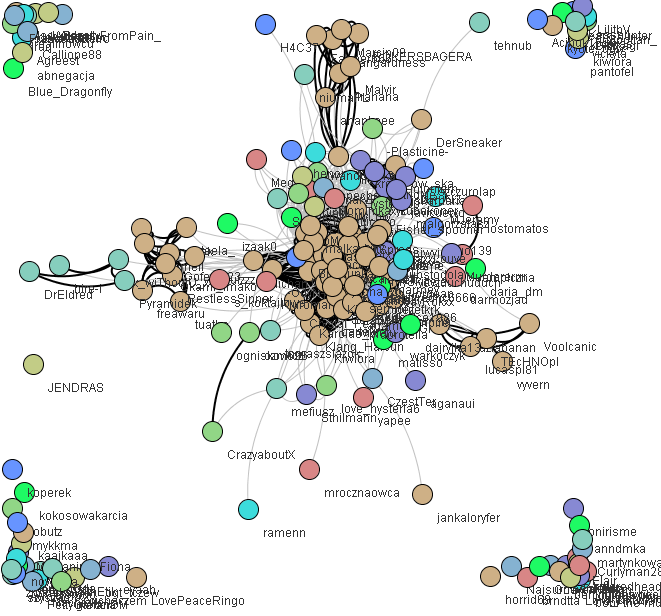
\includegraphics[scale=0.5]{wyniki/final200Events/2200events.png}
\end{figure}

\begin{figure}[H]
\centering
\caption{Histogram PageRank, $\frac{2}{5}$ usuniętych krawędzi}
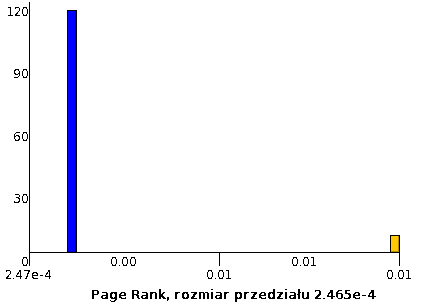
\includegraphics[scale=0.6]{wyniki/final200Events/2200eventsPRHist.png}
\label{fig:1200lovedPRHist}
\end{figure}


\begin{figure}[H]
\centering
\caption{Histogram Betweenness Centrality $\frac{2}{5}$ usuniętych krawędzi}
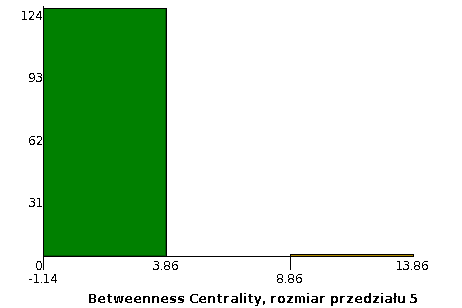
\includegraphics[scale=0.6]{wyniki/final200Events/2200eventsBCHist.png}
\end{figure}


\begin{table}[H]
  \caption{Miary grafu koncertów po usunięciu $\frac{2}{5}$ krawędzi}
  \centering
    \begin{tabular}{cccc}
    \addlinespace
    \toprule
    Miara & Średnia  & Odchylenie standardowe \\
    \midrule
    Liczba znajomych & 10.47 & 13.32 \\
    PageRank & 0.0050 & 0.0045 \\
    BetweennessCentrality & 2.795 & 7.84\\ 
    \bottomrule
    \end{tabular}
  \label{tab:addlabel}
\end{table}

Usunięcie $\frac{2}{5}$ połączeń między użytkownikami doprowadziło do powstania 124 klastrów. 

\subsubsection {$\frac{3}{5}$ krawędzi}

  Kolejne ilustracje oraz tabele prezentują wynik klastrowania grafu pozbawionego  $\frac{3}{5}$  krawędzi.
\begin{figure}[H]
\centering
\caption{Graf koncertów po usunięciu $\frac{3}{5}$ krawędzi}
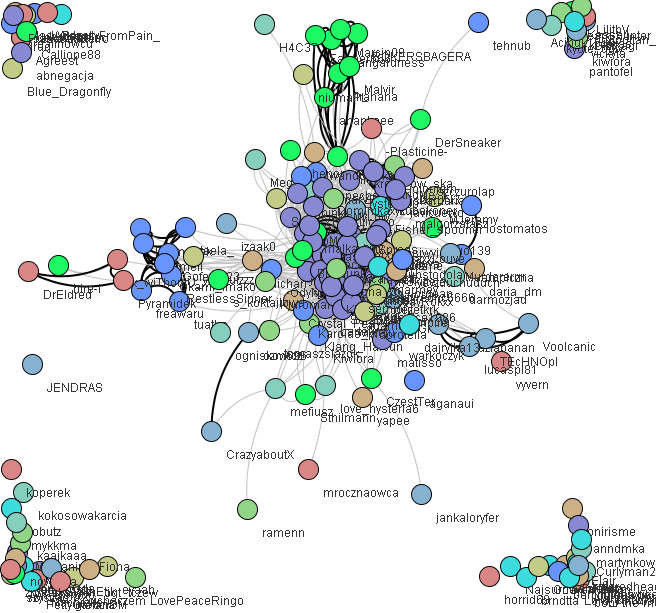
\includegraphics[scale=0.5]{wyniki/final200Events/3200events.png}
\end{figure}

\begin{figure}[H]
\centering
\caption{Histogram PageRank, $\frac{3}{5}$ usuniętych krawędzi}
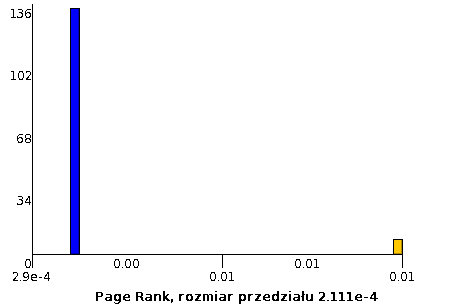
\includegraphics[scale=0.6]{wyniki/final200Events/3200eventsPRHist.png}
\label{fig:1200lovedPRHist}
\end{figure}


\begin{figure}[H]
\centering
\caption{Histogram Betweenness Centrality $\frac{3}{5}$ usuniętych krawędzi}
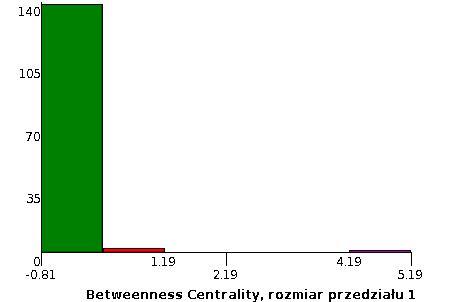
\includegraphics[scale=0.6]{wyniki/final200Events/3200eventsBCHist.png}
\end{figure}


\begin{table}[H]
  \caption{Miary grafu koncertów po usunięciu $\frac{3}{5}$ krawędzi}
  \centering
    \begin{tabular}{cccc}
    \addlinespace
    \toprule
    Miara & Średnia  & Odchylenie standardowe \\
    \midrule
    Liczba znajomych & 10.47 & 13.32 \\
    PageRank & 0.0050 & 0.0048 \\
    BetweennessCentrality & 0.83 & 2.17\\ 
    \bottomrule
    \end{tabular}
  \label{tab:addlabel}
\end{table}

Usunięcie $\frac{3}{5}$ połączeń między użytkownikami doprowadziło do powstania 142 klastrów. 

\subsubsection {$\frac{4}{5}$ krawędzi}

  Kolejne ilustracje oraz tabele prezentują wynik klastrowania grafu pozbawionego  $\frac{4}{5}$  krawędzi.
\begin{figure}[H]
\centering
\caption{Graf koncertów po usunięciu $\frac{4}{5}$ krawędzi}
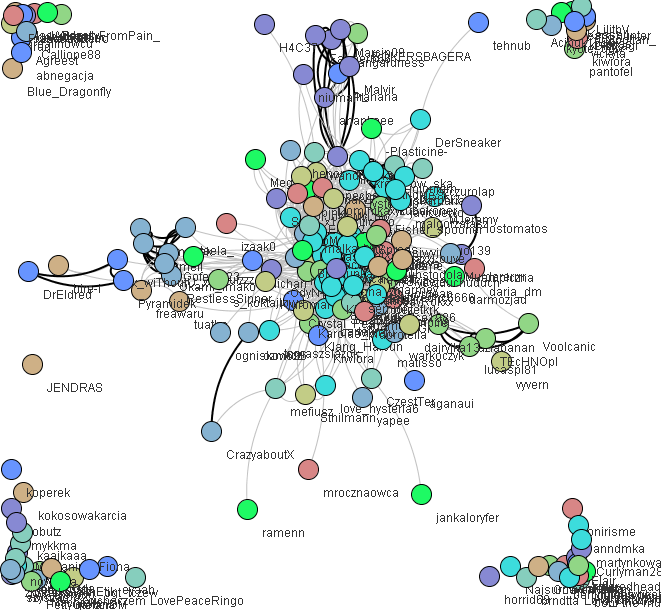
\includegraphics[scale=0.5]{wyniki/final200Events/4200events.png}
\end{figure}

\begin{figure}[H]
\centering
\caption{Histogram PageRank, $\frac{4}{5}$ usuniętych krawędzi}
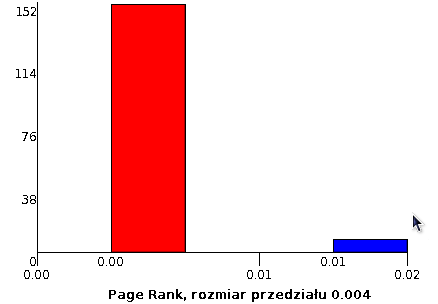
\includegraphics[scale=0.6]{wyniki/final200Events/4200eventsPRHist.png}
\label{fig:1200lovedPRHist}
\end{figure}


\begin{figure}[H]
\centering
\caption{Histogram Betweenness Centrality $\frac{4}{5}$ usuniętych krawędzi}
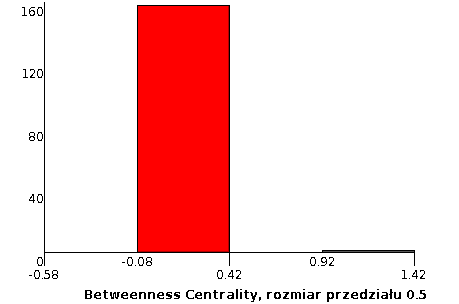
\includegraphics[scale=0.6]{wyniki/final200Events/4200eventsBCHist.png}
\end{figure}


\begin{table}[H]
  \caption{Miary grafu koncertów po usunięciu $\frac{4}{5}$ krawędzi}
  \centering
    \begin{tabular}{cccc}
    \addlinespace
    \toprule
    Miara & Średnia  & Odchylenie standardowe \\
    \midrule
    Liczba znajomych & 10.47 & 13.32 \\
    PageRank & 0.0050 & 0.0051 \\
    BetweennessCentrality & 0.11 & 0.44\\ 
    \bottomrule
    \end{tabular}
  \label{tab:addlabel}
\end{table}

Usunięcie $\frac{4}{5}$ połączeń między użytkownikami doprowadziło do powstania 159 klastrów. 

\subsubsection {Wnioski}
  Usunięcie częsci krawędzi w tym grafie spowodowało utworzenie się kilku wyraźnych klastrów, zawierających większe ilości użytkowników.
Spora ilość klastrów zawierających tylko jednego użytkownika świadczy o dużej ilości pojedynczych połaczeń między wierzchołkami grafu.
Spowodowane jest to ogromną ilością koncertów, które mogą połączyć użytkowników. 



\section{Wnioski}
Przeanalizowaliśmy sieć społecznościowa last.fm pod względem trzech
rodzajów połączeń: znajomych, koncertów i ulubionych.

Klastrowanie znajomych dało najlepsze wyniki. Na podstawie
eksperymentów określiśmy najlepszy parametr klastrowania. W przypadku
usuwania 2/5 krawędzi tworzy się kilka wyraźnych grup
wieloużytkownikowych i niewiele grup o małej liczebności. Usuwanie
mniejszej liczby krawędzi prowadzi do powstawania małej liczby dużych
grup, natomiast usuwanie większej liczby krawędzi doprowadziło do
wydzielenia się gigantycznej liczby mikro społeczności.

Wyniki analizy grafów utworów ulubionych i koncertów były mniej udane,
w miarę zwiększania liczby usuwanych krawędzi struktury
społecznościowe nie zaczęły się pojawiać. Odcinanie kolejnych krawędzi
doprowadzało do odłączania się użytkowników od głównej grupy.
Częściowo jest to spowodowane sposobem tworzenia połączeń w grafie,
waga połączenia była taka sama niezależnie od liczby wspólnych utworów
lub koncertów. Ponad to, struktura połączeń ulubionych była rzadka w
przypadku analizowania tylko 100 użytkowników, co było robione ze
względy na wydajność pakietu Jung.

Podsumowując, wyniki analizy znajomych były zgodne z naszymi
oczekiwaniami, natomiast klastrowanie ulubionych utworów i koncertów
nie wygenerowało zbyt interesujących wyników.

\section{Rozwój}

W dalyszych etapach prac konieczna jest zmiana sposobu tworzenia grafu
na taki który umożliwi uwzględnienie wag krawędzi oraz zmiana
alagorytmu klastrującego na taki który wydajniej przetwarzałby duże
ilości danych.

Dodatkowe prace mogłyby polegać na porównaniu wyników róznych
algorytmów klastrowania lub na analizie innych powiązań z serwisu
last.fm.


\section {Dokumentacja kodu}
\subsection{Pakiet analysis}
W tej części projektu znajdują się kod umożliwiający tworzenie oraz analizowanie sieci społecznych.
\begin{itemize}
\item AnalysisHelper – klasa wspomagająca wyszukiwanie części wspólnych społeczności
\begin{itemize}
\item ExtractSolidCommunities – metoda zwracająca części wspólne dwóch wyników klastrowania
\item ExtractSolidCommunitiesFactor – służy do określania współczynnika pokrycia
\end{itemize}
\item EvParams – klasa opisująca parametry okresy klastrowania koncertów
\item GraphFactory – klasa zwierająca metody umożliwiające tworzenie grafów różnego rodzaju oraz raportowanie wyników
\begin{itemize}
\item CreateEventsGraph – tworzenie grafu powiązań koncertowych, można określić liczbę użytkowników oraz parametr okresu poprzez klasę EvParams
\item CreateFriendsGraph – tworzenia grafu sieci na podstawie informacji o znajomych
\item CreateLovedGraph – tworzenie  grafu na podstawie ulubionych utworów użytkowników
\item Report – generowanie raportu opisującego każdy klaster i każdego użytkownika
\end{itemize}
\item MathHelper – Klasa zawiera metody pomocnicze do obliczania średniej oraz odchylenia standardowego.
\item TextModeAnalyzer – Klasa służąca do uruchamiana analiz w trybie tekstowym.
\item UserLabeller – Klasa która etykietuje użytkowników w wizualizacji
\item VisualAnalyzer – Analizator w trybie graficznym
\end{itemize}

\subsection{Pakiet crawler}
Pakiet ten zawiera klasy służące do pobierania danych z serwisu Last.fm.
\begin{itemize}
\item Crawler – zawiera informacje o kluczu API last.fm 
\item EventCrawler – pobiera koncerty oraz ich uczestników
\item LovedCrawler – pobiera ulubione utwory użytkowników
\item UserCrawler – pobiera znajomych
\end{itemize}
\subsection{Pakiet hiberex}
Klasy pakietu hiberex odpowiedzialne są za mapowanie danych z bazy danych.
\begin{itemize}
\item AdditionalFunc – klasa zawierająca metody uproszczające zapytania do bazy danych
\item SessionFactoryUtil  - fabryka sesji, niezbędna do działania hibernate
\item Klasy odpowiadające rekordom w bazie danych
\begin{itemize}
\item Shout
\item User
\item Artist       
\item Pair 
\item Tag          
\item Venue
\item Event 
\item Playlist 
\item Group   
\item Track
\end{itemize}
\end{itemize}

\begin{thebibliography}{99}   
\bibitem{cipka}{Community structure in social and biological networks” http://www.pnas.org/content/99/12/7821.full.pdf}
\bibitem{hujek}{„JUNG” http://jung.sourceforge.net/}
\end{thebibliography}

\end{document}



